\section{Simulation der Steuerungsaufgabe von Quadrokoptern}
Die Popularität von unbemannten Flugzeugen im letzten Jahrzehnt nahm besonders im Bereich der Quadrokopter zu, sodass durch die sinkenden Kosten von Sensorik und Minicomputern, zahlreiche zukunftsträchtige Ergebnisse und Anwendungen erforscht worden sind. \footcite[Vgl.][S. 1]{Koch.2018}
Anwendungsgebiete beinhalten z.B. die Landwirtschaft, den Pakettransport oder die Überwachung von großflächiger Infrastruktur wie Stromnetze. \footcite[Vgl.][S. 1]{Deshpande.2020}
Eine Simulation von unbemannten Flugzeugen stellt eine Flugumgebung und vielseitige Sensorik bereit und kann je nach Anwendung Effekte wie Wind, Wolken und Niederschlag einbeziehen. \footcite[Vgl.][S. 1496]{Hentati.2018}

\subsection{Flugdynamiken eines Quadrokopters}
Die Simulation des Quadrokopters stellt eine Simulation eines Flugkörpers mit drei Rotations- und drei Translationsbewegungen und demnach insgesamt sechs verschiedenen Freiheitsgraden dar. \footcite[Vgl.][S. 2]{Koch.2018}
Ein Quadrokopter ist ein fester Körper mit vier befestigten Rotoren, welche sich ausschließlich in eine Richtung drehen und positiven Schub in die Z-Achse des Körpers ausüben können. \footcite[Vgl.][S. 3]{Molchanov.2019}
Die vier Rotoren werden als + oder X Konfiguration entweder direkt in Richtung der X- und Y-Achse (+), oder um 45° gedreht (X) an der Drohne befestigt. \footcite[Vgl.][S. 2]{Koch.2018}
Jede Bewegung der sechs verschiedenen Arten wird durch die unterschiedliche Steuerung, der im Fall des Quadrokopters, vier Rotoren getätigt.
Eine unterschiedliche Ansteuerung der Rotoren und den demnach verschieden starken Auftrieben resultiert in den drei Rotationsbewegungen Rollen, Nicken und Gieren. \footcite[Vgl.][S. 2]{Koch.2018}
\begin{figure}[htb]
    \centering
    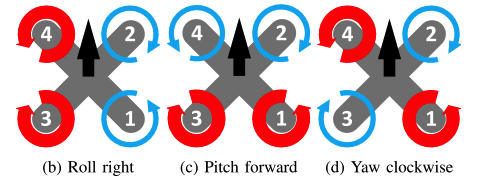
\includegraphics[height=3cm]{lib/graphics/Drone axis.png}
    \caption[Rotationsbewegungen eines Quadrokopters]{Rotationsbewegungen eines Quadrokopters\footnotemark}
    \label{abb:drone axis}
\end{figure}
\footnotetext{Enthalten in: \cite[][S. 2]{Koch.2018}}

Rollen wird wie aus Abbildung drei hervorgeht durch unterschiedlichen Auftrieb der zwei linken und rechten Rotatoren, das Nicken durch Unterschiede der vorderen und hinteren Rotatoren hervorgerufen.
Das Gieren bzw. die Rotation um die Z-achse wird durch die stärkere Rotation der sich im Uhrzeiger drehenden oder der sich gegen den Uhrzeiger drehenden Rotoren bewerkstelligt. 

Diese Rotationsbewegungen werden mathematisch als Matrix der Eulerschen Winkel repräsentiert, welche die Folge der einzelnen Drehungen entlang der X-, Y-, und Z-Achse enthält. \footcite[Vgl.][S. 3]{Deshpande.2020}
Das Zusammenspiel dieser Rotationsbewegungen, dargestellt anhand Formel vier, mit der durch die Rotatoren entlang der Z-Achse der Drone erzeugte Schubkraft und den Rollraten, beschrieben in Formel fünf, sorgt für die Bewegung der Drohne in Richtung der zukünftigen Koordinaten nach Formel sechs. \footcite[Vgl.][S. 2]{Deshpande.2021}

\begin{description}
    \item \begin{center} (4) $R = \begin{pmatrix} C_{\psi}C_{p} & S_{\xi}S_{p}C_{\psi} - S_{\psi}C_{\xi} & S_{\xi}S_{\psi}+S_{p}C_{\xi}C_{\psi} \\ S_{\psi}C_{p} & S_{\xi}S_{\psi}S_{p} + C_{\xi}C_{\psi} &  -S_{\xi}C_{\psi} + S_{\psi}S_{p}C_{\xi}\\ -S_{p} & S_{\xi}C_{p} & C_{\xi}C_{p} \end{pmatrix}$ \end{center}
\end{description}
In Formel vier wird der Rotationszustand der Drohne zu den Weltachsen durch die Sinus- und Cosinuswinkel $S_{a}$ und $C_{a}$ repräsentiert, wobei für $a$ die Art der Rotation also Rollen $(\xi)$, Nicken $(p)$ und Gieren $(\psi)$ eingesetzt wird. \footcite[Vgl.][S. 2]{Deshpande.2021}
\begin{description}
    \item \begin{center} (5) $I\begin{pmatrix} \dot p \\ \dot q \\ \dot r\end{pmatrix} = \begin{pmatrix} l(F_{1} + F_{2} - F_{3} - F_{4}) \\ l(-F_{1} + F_{2} + F_{3} - F_{4}) \\ -M_{1} + M_{2} - M_{3} + M_{4}\end{pmatrix} - \begin{pmatrix} p \\ q \\ r \end{pmatrix} \times I\begin{pmatrix} p \\ q \\ r \end{pmatrix}$ \end{center}
\end{description}
Formel fünf inkludiert in der Matrix $I$ die Trägheitsmomente um die X-, Y- und Z-Achsen in Abhängigkeit der Rollrate $p$, Nickrate $q$ und Gierrate $r$. \footcite[Vgl.][S. 2]{Deshpande.2021}
Der Schub der in der Länge $l$ vom Schwerpunkt entfernten Rotatoren wird mittels $F_{i}$ und das Drehmoment mit $M_{i}, \forall i \in \{1,2,3,4\}$ gekennzeichnet. \footcite[Vgl.][S. 3]{Deshpande.2020}
\begin{description}
    \item \begin{center} (6) $m\begin{pmatrix} \ddot x \\ \ddot y \\ \ddot z \end{pmatrix} = \begin{pmatrix}0 \\ 0 \\ -mg\end{pmatrix} + R\begin{pmatrix} 0 \\ 0 \\ \sum_{i=1}^{4} F_{i} \end{pmatrix}$ \end{center}
\end{description}
Weiterhin ist die Beschleunigung $\ddot x$, $\ddot y$ und $\ddot z$ in Richtung der drei Achsen durch die Masse $m$ und die Gravitation $g$ beeinflusst. \footcite[Vgl.][S. 3]{Deshpande.2020}

%\subsection{Quadrokopter im Kontext von RL}

\subsection{Existierende Simulationen von Quadrokoptern}

\textit{RotorS}

Die Simulationsumgebung RotorS wurde auf Basis des Robot Operating Systems (ROS) entwickelt, um Programmtestzeiten zu verkürzen, Fehlersuche zu vereinfachen und Unfälle mit echten Mikroflugzeugen zu vermindern. \footcite[Vgl.][S. 596]{Furrer.2016}
Dabei wurde die Simulation modular entworfen, sodass Komponenten wie Steuerung oder Zustandsschätzung austauschbar sind und das Hinzufügen von neuen Drohnen erleichtert wird. \footcite[Vgl.][S. 595]{Furrer.2016}
Die Komponenten der Drohne stellen dabei Plug-ins der verwendeten Gazebo Physik-Engine dar, wodurch ein Mikroflugzeug aus den Teilen des Körper, der Anzahl der Rotoren und Sensorik an fixen Position zusammengesetzt wird. \footcite[Vgl.][S. 597]{Furrer.2016}
Mittels der standardmäßigen Sensorik können Informationen über die direkte und visuell gemessene Trägheit sowie über die Wegbestimmung erzielt werden. \footcite[Vgl.][S. 597]{Furrer.2016}
Anstelle des Wegbestimmungssensors kann auch eine Komponente zur Zustandsschätzung für hochfrequente Abragen implementiert werden. \footcite[Vgl.][S. 598]{Furrer.2016}
Die Steuerungskomponente wird durch eine einfache Schnittstelle einer geometrischen Steuerung bedient, welche Aktionen in Form von Rotationswinkeln, Höhen oder Positionen entgegen nimmt. \footcite[Vgl.][S. 598]{Furrer.2016}

\textit{CrazyS}

CrazyS stellt eine Erweiterung der Simulation RotorS auf Basis desselben ROS, um die Modellierung des Nano-Quadrokopters Crazyflie samt ihrer Dynamik ihres Kontrollsystems und ihrer Sensorik dar. \footcite[Vgl.][S. 81]{Silano.2020}
Mit der Modellierung der Nanodrohne wurde gleichzeitig ein Konzept zur Erweiterung der RotorS Fähigkeiten dargelegt sowie die Entwicklung von Software-in-the-Loop (SITL) als nahezu Echtzeitüberwachung vorangetrieben. \footcite[Vgl.][S. 82]{Silano.2020}

\textit{AirSim}

AirSim ist eine open-source Simulationsplattform, mit der das Ziel verfolgt wird, durch eine detailreiche Simulation die Entwicklung von RL und anderen Methoden des maschinellen Lernens voranzutreiben \footcite[Vgl.][S. 2]{Shah.2017}
Zur Modellierung der Simulationsphysik wird die Unreal Engine 4 aufgrund ihres hohen Grades an physikalischer und visueller Realität eingesetzt. \footcite[Vgl.][S. 1]{Shah.2017}
Der Aufbau der Simulation folgt einem modularen Entwurf, welcher unter anderem die einzelnen Komponenten Fahrzeug, Umgebung, Physik-Engine, Sensorik und Darstellungsschnittstelle beinhaltet. \footcite[Vgl.][S. 3]{Shah.2017}
Die Schnittstelle des Fahrzeugs erlaubt eine Steuerung über viele Betätigungselemente und deren Eigenschaftsparameter wie Masse, Trägheit, Widerstand oder Reibung. \footcite[Vgl.][S. 5]{Shah.2017}
Ein Fahrzeug ist dabei durch die Umgebungskomponente beeinflusst, welche physikalische Effekte wie Gravitation, Luftwiederstand, Luftdruck und magnetische Felder simuliert. \footcite[Vgl.][S. 6]{Shah.2017}
Die Umgebung wird für das Fahrzeug wahrnehmbar durch die Modellierung von Sensoren wie GPS, Beschleunigungsmesser, Gyroskop, Barometer und Magnetometer. \footcite[Vgl.][S. 9]{Shah.2017}

%\textbf{Text zur Physik-Engine und zum Rendering noch möglich}

\textit{gym-pybullet-drones}

Eine weitere nach der Gym Schnittstelle definierte Simulationsumgebung ist gym-pybullet-drones. \footcite[Vgl.][S. 1]{Panerati.332021}
Basierend auf der Bullet Physik-Engine ermöglicht die Simulation unter anderem das visuell basierte Training von mehreren Agenten mittels RL unter realistischer Modellierung von Kollisionen und aerodynamischen Effekten. \footcite[Vgl.][S. 1]{Panerati.332021}
Die Wahl der Physik-Engine wurde aufgrund des CPU und GPU basierenden Renderings, des Kollisionsmanagements und der Kompatibilität mit dem Unified Robot Description Format (URDF) getroffen \footcite[Vgl.][S. 3]{Panerati.332021}
Durch die Kompabilität mit dem URDF Format kann die standardmäßige Simulation des Drohnenmodells Bitcraze Crazyflie 2.x um weitere Nanoquadrokopter erweitert werden. \footcite[Vgl.][S. 3]{Panerati.332021}